
% Chapter 3
% ======================================================================================================
% NOTES, TODOS

% ======================================================================================================

\chapter{Lightweight Cryptography Solution for (I)IoT-DT Communication}
\label{Chapter3} % For referencing the chapter elsewhere, use \ref{Chapter1} 



In the preceding chapter, the comprehensive examination of existing literature demonstrated that the majority of authors either presume the security of data transmitted from IoT sensors or recommend employing cryptographic methods like AES, SHA-256, and RSA to ensure a secure communication channel. However, applying such mechanisms on a resource-constrained device is unfeasible due to their substantial demands in terms of computation, memory, and power consumption \cite{vanderwalSecuringNetworksIoT2022a}

% In the previous chapter, the systematic literature review revealed that most of the authors either assume data communicated from IoT sensors are secure  or they suggest using AES, SHA-256, and RSA cryptography solutions to secure the communication channel. Implementing such mechanisms on a resource-constrained device however is impractical as these cryptographic solutions demand high resources in terms of computation, memory, and power. 



% The primary aim of this chapter is to respond to research question 3, which centers on enhancing the security of the communication channel between Digital Twin and resource-constrained (I)IoT devices. To tackle this issue, we present a proposed solution, which is a communication scheme involving the encryption of the data and authentication of the components using one of NIST's standardized lightweight algorithms known as ASCON.

The primary aim of this chapter is to respond to research question 3, which focuses on securing the communication channel between Digital Twin and resource-constrained (I)IoT devices. To address this challenge, we proposed a solution (a communication scheme) that involves both encrypting and authenticating data communicated using one of NIST's standardized lightweight algorithms known as ASCON.  

Before diving into the implementation detail and the experiment outcome, a foundational background is provided in the subsequent section for components and concepts relevant to the proposed solution. 



\section{Preliminaries}
% The following section was part of preliminary 
The implementation part of the proposed solution has four main components worth to describe them here. These are Digital Twin, (I)IoT devices, lightweight encryption algorithms, and MQTT protocol. This section serves as a foundation by providing background information for the aforementioned components.



\subsection{Digital Twin and Industry 4.0}
Digital Twin is an integrated software solution with modelling, analytical capability, and interconnectivity technology to replicate the physical world in digital space. The inception of this concept can be traced back to NASA's work on the Apollo 13 space project in 1970, where it was used as 'mirror systems' to troubleshoot and resolve issues \cite{adrienbacueDigitalTwinsEnhanced2022}. However, it was in 2002, the term "Digital Twin" coined for the first time by Michael Grieves and John Vickers of NASA in 2003, specifically for the application of product life cycle management \cite{jones_characterising_2020}.

The concept and definition of Digital Twins have been open to various interpretations, depending on the specific context.  However, through our systematic literature review in chapter \ref{Chapter2}, we identified Digital Twins typically revolve around three fundamental components: \textbf{states} (physical and digital), \textbf{interconnectivity} (communication channel between the physical and virtual state) and \textbf{process} (a mechanism for processing and analysing data). 

\begin{figure}[H]
    \centering
    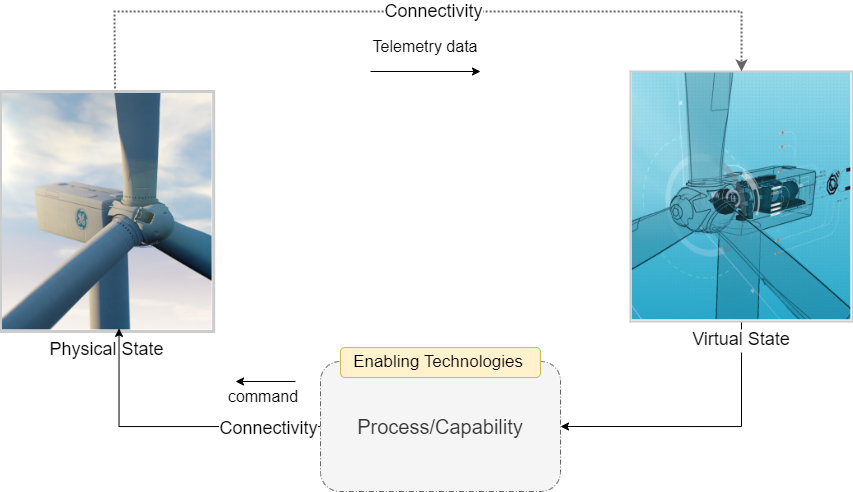
\includegraphics[width=1\linewidth]{images/fp/digital-twin-concept.drawio.png}
    \caption{Three Component of Digital Twin--State, Connectivity, and Capability(Process)}
    \label{fig:dt-concept}
\end{figure}

% Here, we provide a comprehensive definition of Digital Twin synthesised from a collection of various definitions of research publications:

% \textit{ Digital Twin is a virtual representation of a physical object, process or system that mirrors its real-world counterpart through real-time updates and tracking of its entire life-cycle. It is designed to model the physical characteristics and behaviours of the object using digital technology, mapping the physical operating environment to virtual space for interaction, and providing valuable insights through collecting asset-centric data, analytic capabilities, and simulations. Digital twins are used to monitor, simulate, optimise and predict the state of a physical object. They have a standard structure, end-to-end connectivity, communication protocol with backward compatibility, and a standard data format for communication between the twins.}

% The definition and respective reference are listed in Table \ref{tbl:dtconcept}


\begin{itemize}
% Virtual replica, Model, Evolving digital profile 
% A process, product, system, environment, industrial assest 
    \item \textbf{State}: Digit Twin has two states (see \ref{fig:dt-concept}); Virtual and Physical state. The virtual state is a digital (software) replica or model representation of a physical object, closely resembling the physical aspect. It can also be described as an evolving digital profile that captures the historical and current status of the represented object \cite{becueCyberFactorySecuringIndustry40with2018}. The physical state, on the other hand, refers to the real-world object of what the Digital Twin represents. The object that is represented by the virtual state could be physical components, processes \cite{wangDTCPNDigitalTwin2022, sousaELEGANTSecurityCritical2021, lopezDIGITALTWINSINTELLIGENT2021, rebecchiDigitalTwin5G2022, luongnguyenDigitalTwinIoT2022}, products, industrial assets \cite{dietzIntegratingDigitalTwin2020, eckhartEnhancingCyberSituational2019}, and environments.

    \item \textbf{Connectivity}: To keep the virtual state with the physical counterpart, a wired or wireless communication channel must be established. To keep the virtual state fidelity, the physical state should send  telemetry data (environmental sensor measurements) in real time. In this regard, wide sensor arrays can be deployed in the physical world to keep the data flow synchronized \cite{danilczykSmartGridAnomaly2021}. On the other hand, a command (a control message) can be sent from the virtual state to the physical state. Furthermore, ensuring a communication protocol that supports backward compatibility and adheres to a standard data format is required for achieving seamless data exchange between the two states \cite{atalayDigitalTwinsApproach2020}.

 
    \item \textbf{Process/Capability}: The true power of Digital Twin lies primarily due to the utilization of enabling technologies\cite{sousaELEGANTSecurityCritical2021}. This aspect also differentiates Digital Twin from simulation software. The use of enabling technology such as machine learning, blockchain, cloud computing, and big data analytics equipped Digital Twin with capabilities for better decision-making and to be used as a security tool. 
    
    Digital Twin can be equipped with enabling technology to provide various security services. For example,  detecting abnormal process events or deliberately injected malicious content \cite{saadImplementationIoTBasedDigital2020}, for prompt intervention and resolution of issues \cite{akbarianSecurityFrameworkDigital2021}, as a cyber situational awareness tool \cite{eckhartEnhancingCyberSituational2019} and so on.  
    
% In most definitions, Digital Twin is intended for simulation. One definition elaborates the simulation function as an insight gained through collecting asset-centric data. In quite a number of definitions, it is also stated that the digital twin is used for monitoring and controlling the real-world counterparts. In one definition the authors argued it can be used to increase cyber situational awareness for Cyber Critical Infrastructures


% In conclusion, Of the three core components of Digital Twin, only the "state" is explicitly described within the definition. The intended purpose and the interconnectivity between the two states are not always included in the provided definition.


    
\end{itemize}


% \begin{table}[H]
% \small
% \centering
% \caption{\label{tbl:dtconcept} Definition of digital twin in the literature}
% % \resizebox{\linewidth}{!}{
% \begin{NiceTabular}{p{10cm}|p{4cm}}
% \CodeBefore
% % \rowcolors[gray]{2}{0.8}{}[cols=1-2,restart]
% \Body
% \toprule
%     \textbf{DT definition} & \textbf{Reference(s)} \\
%     \midrule
%      Digital twins are virtual representations of industrial assets that provide valuable insights through collecting asset-centric data, analytic capabilities and simulations & \cite{dietzIntegratingDigitalTwin2020, eckhartEnhancingCyberSituational2019} \\  
%      \hline
%     A system that continuously monitors the physical state of an environment through wide sensor arrays and compares it to simulation models to gain deeper insights into its operating condition & \cite{williamdanilczykANGELIntelligentDigital2019, danilczykSmartGridAnomaly2021, veledarDigitalTwinsDependability2019, kumarBlockchainDeepLearning2022, hadarCyberDigitalTwin2020} \\
%     \hline
%     A virtual representation of a physical system, process or product that is synchronized with its real-world counterpart & \cite{gehrmann_digital_2020, luongnguyenDigitalTwinIoT2022, lopezDIGITALTWINSINTELLIGENT2021, rebecchiDigitalTwin5G2022} \\ 
%     \hline
%     A technology to map the physical operating environment to virtual space for interaction. & \cite{wuDeepLearningDriven2022}  \\ 
%     \hline
%     Evolving digital profile of the historical and current value of physical object or process & \cite{becueCyberFactorySecuringIndustry40with2018} \\
%     \hline

%     Virtual representation of physical objects or systems that can be used to monitor and control the real-world counterparts & \cite{almeaibedDigitalTwinAnalysis2021, chukkapalliCyberPhysicalSystemSecurity2021, dietzEmployingDigitalTwins2022}\\
%     \hline
%     virtual replica of physical object with standard structure, end-to-end connectivity, communication protocol with backward compatibility, and standard data format for communication between the twins & \cite{atalayDigitalTwinsApproach2020} \\

%     % \hline
%     % This paper is rejected
%     % DT is a mapping between physical object and virtual entity that receive data in real-time to predicate the state of the physical object & \cite{dinglingsuzehuiquDetectionDDoSAttacks2022} \\
    
%     \hline
%     A virtual Model designed to accurately map a physical object or process & \cite{wangDTCPNDigitalTwin2022, sousaELEGANTSecurityCritical2021} \\
    
%     \hline
%     a method to describe and model the physical characteristics and behaviors of physical objects by using digital technology & \cite{wangSoCbasedDigitalTwin2020} \\
    
%     \hline
%     A virtual space for representation of real world object and an information flow to keep them synchronize  & \cite{giovannipaolosellittoEnablingZeroTrust2021}\\
    
%     \hline
%     A digital twin is a virtual representation of a physical object that tracks and mimics its entire life-cycle through real-time updates & \cite{vargheseDigitalTwinbasedIntrusion2022, dietzUnleashingDigitalTwin2020} \\
    
%     \hline
%     Digital Twin is a virtual replica of physical system that precisely mirror the internal behavior of system for monitoring, simulating, optimizing and predicating the state of the system & \cite{akbarianSecurityFrameworkDigital2021, akbarianIntrusionDetectionDigital2020} \\
    
%     \hline
%     a digital twin is defined as an integrated system that combines computational, communication and physical aspects of Cyber Critical Infrastructures (CCIs) to provide increased cyber situational awareness & \cite{salviCyberresilienceCriticalCyber2022, pirbhulalNovelFrameworkReinforcing2022} \\
% \bottomrule
% \end{NiceTabular}
% % }
% \end{table}

% The definition presented in the table  \ref{tbl:dtconcept} is interpreted using the three components(State, Connectivity, Process) as follows.  


\subsection{Internet of Things and Industry 4.0 }
IoT and (I)IoT are related technologies where their difference relies only on their application area. While IoT is in IT and home environments,  IIoT is an application of IoT in the manufacturing industry \cite{boyes_industrial_2018}. In other words, it emerges from IoT \cite{fuller_digital_2020} to support the optimization of operations in industrial environments. Sensors, actuators and RFID are an instance of (I)IoT in the context of Industry 4.0. These technologies play a vital role in bridging the gap between the business IT environment and the operation environment in OT (operational technology) \cite{adrienbacueDigitalTwinsEnhanced2022}.


Though (I)IoT enhances control and visibility in industrial operations, it also introduces new attack surfaces as evidently shown by a study that reveals an increase in attacks like Stuxnet, flam, and Doqu on critical infrastructure as more SCADA systems communicate over TCP/IP communication channels \cite{eden_scada_2017}. And, Boyes et al. \cite{boyes_industrial_2018} point out that (I)IoT devices, such as sensors, actuators, and RFID tags, have limited power, storage, and processing capacity to support strong encryption mechanisms and effectively secure the communication channel. This is where our research contribution comes into play, addressing this challenge by implementing a lightweight cryptography-based communication scheme using a payload encryption technique.

\subsection{ESP31 - Wemos Lolin32 Lite}

The Wemos LOLIN32 Lite is a low-cost, low-power system on a chip (SoC)  microcontroller that is popular for Internet of Things (IoT) projects. It is based on the ESP32 SoC, which has a 32-bit dual-core processor, 4MB of flash memory, and 520kB of RAM \cite{noauthor_espressif_systems_01292021_esp32-1991551pdf_nodate}. The LOLIN32 Lite also has Wi-Fi and Bluetooth connectivity, making it ideal for this project as the implementation in this project involves sending and receiving data to and from Digital Twin through a wireless link. According to the datasheet of esp32 from espressive system, the board is low power consumption which can be used various application areas including industrial automation, health care and smart home \cite{noauthor_espressif_systems_01292021_esp32-1991551pdf_nodate}. 

The board is shipped with essential components for (I)IoT projects (see Figure \ref{fig:esp32}). At the centre, we have Xtensa microprocessors with 2 cores of 240 MHz clock frequency. It is equipped with 4MB of flash memory and it can also support external flash up 16MB. It has a number of GPIO (General Purpose Input/Output) pins for various functions. Among these, we leverage the GPIO 17 for data logging to an external power measurement unit (for further insights, refer to  Chapter \ref{Chapter4} Section \ref{sec:power})
Furthermore, two LEDs; one for the power charge indicator and the other for the GPI022 pin indicator are mounted. In addition, it supports USB connector for debugging and development with the help of UART CH340C USB-to-serial converter IC(Integrated Circuit).
\begin{figure}[H]    
{
    \centering
    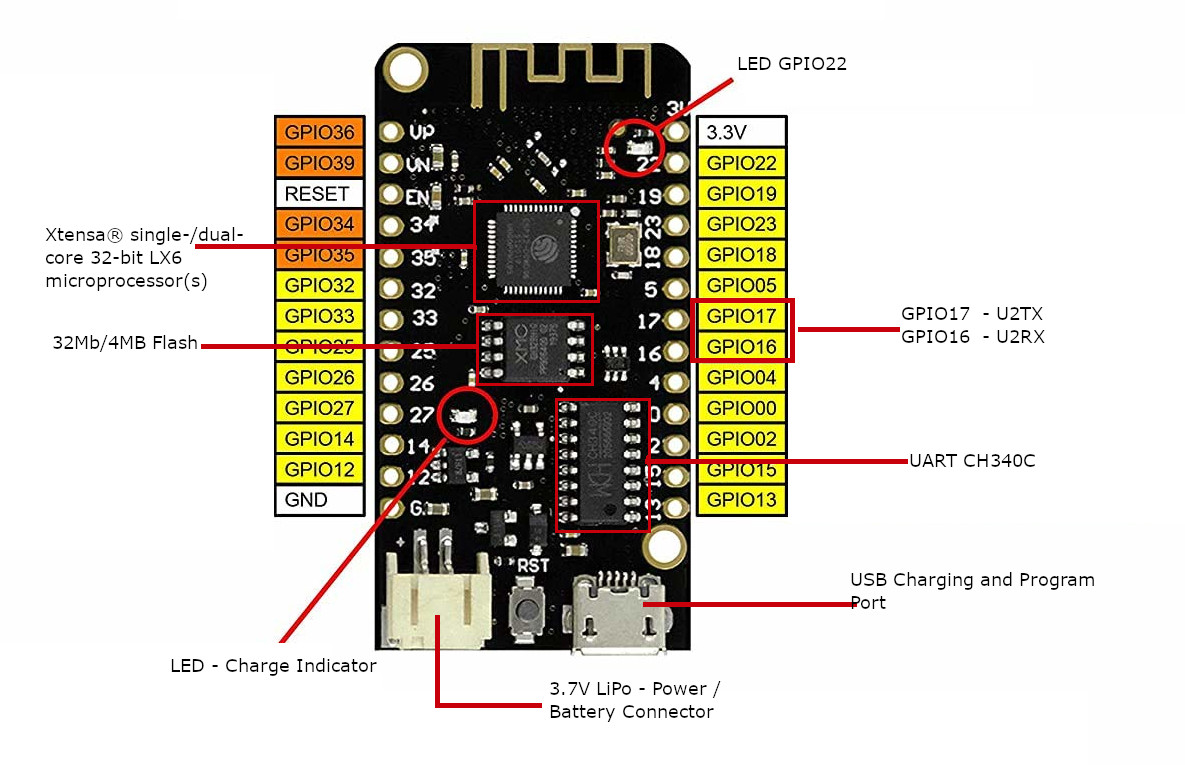
\includegraphics[width=0.99\textwidth]{images/fp/esp32final_edited.jpg}
    \caption{ESP32 Low-power Board From Espressif System}
    \label{fig:esp32}
}
\end{figure}

% \begin{table}[H]
%     % \tiny
%     \centering
%     \caption{\label{tbl:esp-spec} Technical Specification of Wemos Lolin32 Lite}
%     % \resizebox{\linewidth}{!}{
%     \begin{NiceTabular}{|p{2.5cm}|p{3cm}|}
%     \CodeBefore
%     % \rowcolors[gray]{2}{0.8}{}[cols=1-2,restart]
%     \Body
%     \toprule
%         Operating voltage &  3.3V \\
%         \hline
%         Supported Battery &	Lipo 3.7V\\
%         \hline
%         Battery Connector & PH-2 2.0mm\\
%         \hline
%         Digital I/O Pins & 22 \\
%         \hline
%          RAM Memory &  512KB\\
%         \hline
%         Clock Speed(Max) &	240MHz \\
%         \hline
%         SPI Flash &	4M Bytes \\
%         \hline
%         Size & 57*25.4mm \\
%     \bottomrule
%     \end{NiceTabular}
%     % }
% \end{table}

One of the key advantages of the Wemos LoLin32 Lite board is that it is supported by both the Arduino and ESP-IDF (Espressif IoT Development Framework) development environments. For our research project, we opted to use the Arduino embedded development framework to implement the ASCON and AES-GCM algorithms using the C and C++ programming languages. In addition, we utilized PlatformIO, an open-source platform for embedded development, to facilitate the building and deployment of our program onto the Wemos LoLin32 Lite board via the serial port.

\subsection{Lightweight Authenticated Encryption With Associated Data }


Lightweight Authenticated Encryption with Associated Data (AEAD) algorithms are designed to efficiently provide both confidentiality and message integrity in a single operation. These algorithms offer a balance between security and performance, making them suitable for securing data both at rest and in motion \cite{el-hajj_analysis_2023}. The confidentiality aspect is achieved through the generated cipher, while authentication or message integrity is ensured through the tag generated during encryption. Upon receipt, the receiver can decrypt the cipher to access the original message and simultaneously verify the tag to ensure that neither the message nor the cipher has been altered during transmission.

\subsubsection*{AES-GCM}

AES-GCM is a family of authenticated encryption with associated data based on AES (Advanced Encryption Standard) and GCM (Galois Counter Mode). It was first presented by David A. McGrew and John Viega \cite{mcgrew_galoiscounter_nodate} in 2005. Since then it has been adopted for various applications including for TLS and IPSec implementation \cite{salowey_aes_2008}.  


\subsubsection*{ASCON}

ASCON is an authenticated encryption algorithm designed and developed by Christoph Dobraunig, Maria Eichlseder, Florian Mendel and Martin Schläffer \cite{dobraunigAsconV1Lightweight2021}. It become very popular after it wins the CASEAR NIST computation. The authors claim the main goal of the algorithm is to provide simplicity, online, security, side-channel robustness, single-pass and lightweight cipher for the resource-constrained device \cite{dobraunigAsconV1Lightweight2021}. It is also a well-performing algorithm for short messages \cite{dobraunigAsconV1Lightweight2021} like for applications to collect environment and operating conditions in industry 4.0

The algorithm can also be used on high-performing machines to provide encryption and decryption for time-critical applications. It can provide 128-bit key security \cite{dobraunigAsconV1Lightweight2021}, surpassing the currently accepted 80-bit security standard.


\begin{figure}[H]
    \centering
    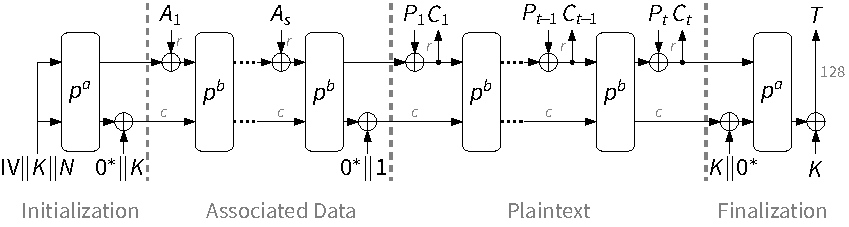
\includegraphics{images/fp/aead_encrypt.pdf}
    \caption{ASCON Encryption Mode of Operation (taken from \cite{dobraunig_ascon_nodate})}
    \label{fig:ascon-enc}
\end{figure}

The encryption and decryption process of ASCON is split into 4 main phases as depicted in Figure \ref{fig:ascon-enc} and \ref{fig:ascon-dec}. These are initialization, associated data processing, plain text/cipher text processing (depending on whether it is in encryption or decryption mod) and finalization. 



\begin{figure}[H]
    \centering
    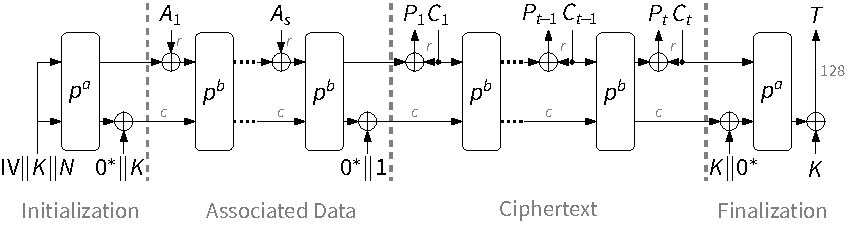
\includegraphics{images/fp/aead_decrypt.pdf}
    \caption{ASCON Decryption Mode of Operation (taken from \cite{dobraunig_ascon_nodate})}
    \label{fig:ascon-dec}
\end{figure}



\subsection{MQTT Protocol }
% What is MQTT
% Why it is important in the field of IoT and industry 4.0
% Key component of MQTT -> publisher, subscribers, and brokers
% lightweight nature of MQTT
% Asynchronous communication and real tim data transfer
% Security measures and authentication mechansims in MQTT

% use case and applicaiton of MQTT

% how we integrate lightweight encryption algorithm in MQTT
% limitation of MQTT

MQTT is a standard messaging protocol for the Internet of Things (IoT), designed and developed by Andy Stanford-Clark (IBM) and Arlen Nipper \cite{bryce_mqtt-g_2018}. It is an extremely lightweight publish/subscribe messaging transport that is ideal for constrained devices, such as microcontrollers and embedded computers \cite{andy_attack_2017}. MQTT is widely adopted in a variety of industries in IIoT systems, including automotive, manufacturing, telecommunications, oil, and gas \cite{atalayDigitalTwinsApproach2020}. 

MQTT protocol is not secure by design to safeguard and protect the data it carries over wire or wireless \cite{andy_attack_2017}. SSL can be used to encrypt the transport layer so that the MQTT header and message are secured. However, this additional security layer requires more resources which may not be available by device-constrained IoT devices. In this work, we show how to use this protocol to transmit an authentic and encrypted message using lightweight payload encryption without adding major additional overhead for the underlying device. 


\begin{figure}[H]
    \centering
    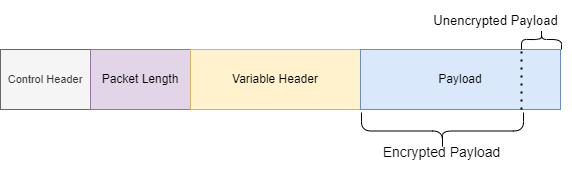
\includegraphics[width=\linewidth]{images/fp/mqttprotocol.drawio.png}
    \caption{MQTT Protocol Header Structure and Payload Encryption}
    \label{fig:mqtt}
\end{figure}

Figure \ref{fig:mqtt} shows the standard MQTT protocol header along with application message payload. Within the MQTT payload section, two distinctive parts can be identified. The first part consists of an encrypted message utilizing one of the AEAD (Authenticated Encryption with Associated Data) encryption family methods. For this particular study, both ASCON and AES-GCM encryption methods are implemented and compared. The second part of the payload contains the associated data. In this context, the device ID serves the purpose of retrieving the appropriate symmetric key by the receiver, thereby ensuring the message's authenticity and integrity.






% ------------------------------Note and Outline------------------------
% 
% The scheme should lightweight 
% The scheme should be secure enough 
% Provide both authentication and encryption 
%  
% 
% ------------------------------End------------------------


\section{Design Consideration and Requirement}
This section outlines the design consideration and requirements that guide the development of our proposed solution (communication scheme) for securing the communication between Digital Twin and (I)IoT. These considerations and requirements are defined primarily in consideration of the resource limitation of (I)IoT devices. 

\subsection{Design Consideration}
Our proposed solution is based on the following design choices that take into account the limited resource (I)IoT devices have.
\begin{itemize}
    \item The scheme should be based on the lightweight application protocol. 
    \item The underlying cryptographic algorithm should be based on a lightweight encryption algorithm standardized by NIST. 
\end{itemize}

\subsection{In Scope Requirements}
\textbf{Performance Requirement}: The proposed solution should be based on a cryptographic algorithm that performs better than traditional algorithms in terms of power consumption, speed, and storage complexity.

\textbf{Security Requirement}: The proposed solution should provide an adequate security level for typical data communication in Industry 4.0 environment. In this regard, an encryption algorithm that provides a minimum 80-bit security level (size of key) should be used. In addition to the above general security requirement, the proposed solution should provide the following security services. 
\begin{itemize}
    \item \textit{Message authentication}: The solution should enable the message receiver to check the authenticity of the message 
    \item \textit{Message Confidentiality}: The solution should provide message confidentiality by encrypting the message. 
    \item \textit{Data Integrity}: The solution should ensure the integrity of data transmission using checksums or other methods to detect message corruption.
    \item \textit{Resilience}: The solution should be capable of detecting man-in-the-middle attacks that involve message modification and data injection. 
\end{itemize}




\subsection{Out of Scope Requirements }
\begin{itemize}
    \item The proposed solution does not have a secure key exchange mechanism between Digital Twin and the physical device. In other words, symmetric keys are assumed to be pre-shared before communication starts. 
    \item The communication protocol (MQTT) at the application level is not encrypted using technologies like SSL/TLS to avoid computation overhead on the constrained device. 
    
\end{itemize}

% These design considerations and requirements are take into 
% proposed communication scheme should meet to be feasible to use in a real-world environment. 





\section{Proposed Solution  }
\label{sec:prosolution}

The (Industrial) Internet of Things ((I)IoT) devices are low-power and resource constrained, which makes them incapable of running traditional cryptographic
schemes such as AES, SHA-256 and RSA. Regardless, these devices are widely used across a range of Industry 4.0 sectors, such as manufacturing, transportation, health, and power
grids, for various applications. In addition, with the emergence of DT in Industry 4.0, (I)IoT sensors are an integral part of Digital Twin technology, in which they are used to collect and send data over wired or wireless channels. Hence, it is crucial to secure the communication between the DT and (I)IoT taking into consideration the limited resource they have. 


In this work, we proposed resource efficient communication scheme based on lightweight cryptographic authenticated encryption to enhance the security of the communication channel between the Digital Twin and its physical components over the MQTT protocol using a technique called payload encryption.


% \subsection{MQTT Payload Encryption/Authentication }

Payload encryption is a technique for ensuring message confidentiality at the application level. In other words, this approach can be used to establish an end-to-end secure channel between the sender and receiver at the application level to provide confidentiality over transmitted data. However, in this paper, we extend the scope beyond message confidentiality and introduce the use of the ASCON, a family of authenticated encryption with associated data (AEAD) algorithms, to provide both message authenticity and confidentiality.

Furthermore, we use the device ID as associative or additional data used along the key and plain text as input for the implementation of the ASCON algorithms. It is important to note that the device ID and its corresponding private key are assumed to be pre-shared between the communicating parties prior to initiating communication. In our case, while the device ID is managed and maintained by the Digital Twin device registration module, the symmetric key should be explicitly configured from both sides (Digital Twin and IoT) of the implementation.  

MQTT protocol is a lightweight messaging protocol that is often used in the Internet of Things (IoT) environment for communication at the application level. This protocol can be configured and programmed to support payload encryption using any encryption algorithm, including the ASCON and AES-GCM (family of AEAD based on AES). 

\begin{figure}[H]
   
    \centering
    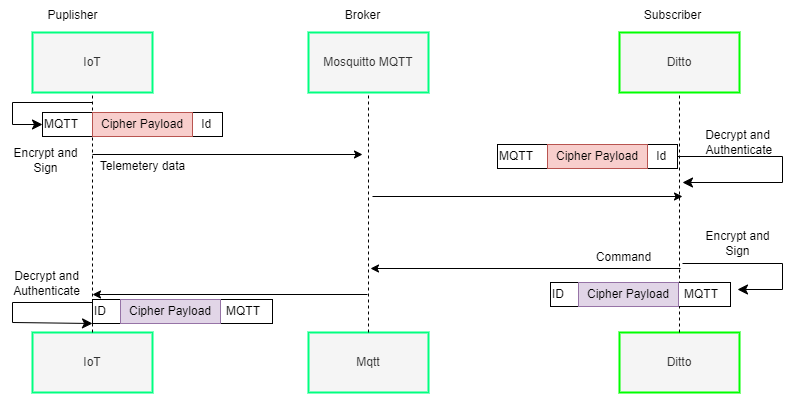
\includegraphics[width=\textwidth]{images/fp/payloadenc.drawio.png}
     \caption{Scheme of Payload Encryption With Authentication Over MQTT Protocol. }
    \label{fig:payload-encauth-schem}
\end{figure}

To achieve payload encryption using ASCON or AES-GCM algorithm over the MQTT protocol, the following steps should be taken. 
\begin{itemize}
    \item[-] \textit{Device ID registration}: Each connected device to Ditto should have a unique device ID. 
    \item[-] \textit{Generate and manage encryption keys}: The device and the Digital Twin agree on a symmetric key. 
    \item[-] \textit{Encrypting and Sending a message}: The sender encrypts the payload of the message along with a tag generated and publishes it to the MQTT broker. The associated data in this case is the unique ID of the device that is sending and receiving data to and from the Digital Twin. 
    \item[-] \textit{Forwarding or Proxing}: The MQTT broker proxies the message through the publisher-subscriber setting. 
    \item[-] \textit{Decryption and Authentication}: The receiver (subscriber) receives the MQTT message and decrypts the payload using a symmetric key retrieved using the device ID of the sender. The receiver then authenticates the payload to ensure that it is from the expected sender and that it has not been tampered with.
    
\end{itemize}

\textbf{\textit{End-To-End Payload Encryption and Authentication:}}
Our communication scheme is based on payload authenticated encryption using one of the AEAD (authenticated encryption with associated data) algorithms over the MQTT protocol. This Implicitly provides end-to-end confidentiality and integrity of a communicated message between Digital Twin and (I)IoT. The Mosquitto broker, which sits between Digital Twin and (I)IoT,  acts as a proxy for forwarding encrypted payload messages. Hence, only the communication parties are able to decrypt and authenticate the payload. 







\section{Implementation Approach}
To validate the applicability and efficacy of our proposed solution (based on lightweight cryptographic algorithms), we conducted an experiment using an ESP32 -- a resource-constrained IoT device -- and Ditto -- an open-source framework for building Digital Twin \footnote{https://eclipse.dev/ditto/}. We opt for ESP32 boards for the experiment due to the fact that they are low-cost and low-power devices in the market \cite{maier_comparative_2017}. Ditto was selected for its ease of customization through Java-based plugins and its widespread use in the open-source community. 



\begin{figure}[H]
    \centering
    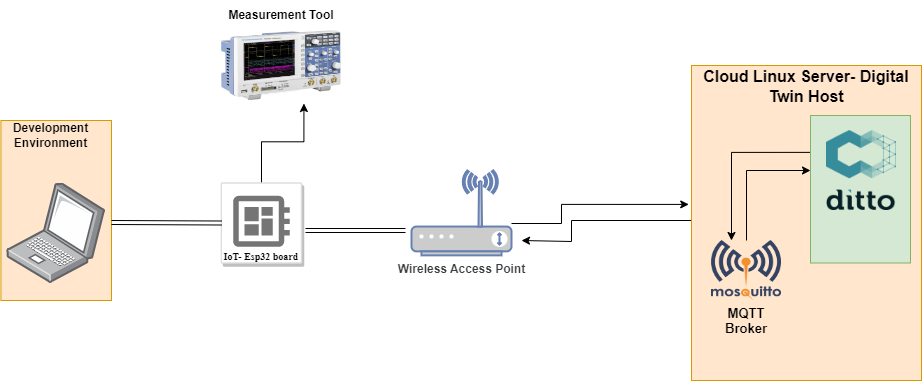
\includegraphics[width=\textwidth]{images/fp/experiment.drawio.png}
    \caption{Research Experiment Setup}
    \label{fig:experiment-setup}
\end{figure}

This section provides a detail of the experimental setup (of Fig \ref{fig:experiment-setup}) and implementation detail of the lightweight encryption/authentication algorithm implemented on both the constrained device and the Digital Twin framework.



% ======================================================================================================
% NOTES, TODOS
% What is Ditto -> reference the official webisite

% ======================================================================================================

\subsection{Eclipse Ditto - Digital Twin Setup}
Eclipse Ditto is an open-source framework for managing IoT devices to create Digital Twin \cite{noauthor_eclipse_nodate}.
It integrates devices via layers like Eclipse Hono and MQTT brokers, allowing managed Digital Twins to connect with various backend systems using protocols such as AMQP, Apache Kafka, HTTP, and MQTT. 

Ditto can be deployed on-premises or in the cloud. For this research, we build and deploy the Ditto code base in the cloud.
In addition, We have two options for deploying and running Ditto on a cloud Linux server. The first option involves utilizing the Kubernetes cluster, which necessitates substantial infrastructure resources. Specifically, a minimum of 4 GB RAM, 8 core processes, and 20 GB disk storage are required. However, the second option, which we have chosen, involves using Docker. This alternative demands fewer resources compared to the previous one. 

Running Ditto in a docker container have seven microservices operating in parallel, each fulfilling distinct functions. These microservices include \textit{Nginx} as the web server, \textit{}, \textit{Ditto Connectivity} for managing the device-to-Ditto connectivity, \textit{Ditto Thing} for managing things (counterpart of physical devices), \textit{Thing Search} for facilitating efficient search using MongoDB, \textit{Swagger-UI} for providing a web-based user interface, and \textit{Ditto Policies} for mainting controlled access over things.

The following steps outline the process required to set up Ditto on a Linux server:

\begin{itemize}
    \item \textbf{Install and Configure Docker:} Begin by installing Docker, a platform for creating and managing containers. Ensure Docker Compose, a utility for defining and running multi-container applications is also installed and configured on your Linux server.
    \item \textbf{Clone Ditto Codebase:} Access the official GitHub repository for Eclipse Ditto and clone the codebase using the command: git clone\texttt{https:// github.com/eclipse-ditto/ditto.git}. 
    \item \textbf{Deploy Ditto Microservices:} Start the Ditto cluster by deploying its microservices in containers. Execute the command: docker-compose up -d. 
    \item \textbf{Check Microservices Status:} verify that all microservices are running and check the health status of Ditto using the following commands: curl -u devops:foobar http://localhost:8080/status/health
\end{itemize}



The process of running Ditto and connecting with the MQTT broker is described below.

\textit{Creating Policy}: In Ditto policies are JSON configuration file that defines who access what. Creating policies is the first step in running Ditto. The policy configuration we use for our project is presented as follows. To speed up experimenting with Ditto we used a bash script that we can run from the terminal of the server. 
\begin{lstlisting}[style=CStyle, caption={A Bash Script of Ditto command To Create Connection}]
#!/bin/bash

curl -X PUT 'http://localhost:8080/api/2/policies/ut.thesis.demo:policy' -u 'ditto:ditto' -H 'Content-Type: application/json' -d '{
    "entries": {
        "owner": {
            "subjects": {
                "nginx:ditto": {
                    "type": "nginx basic auth user"
                }
            },
            "resources": {
                "thing:/": {
                    "grant": [
                        "READ","WRITE"
                    ],
                    "revoke": []
                },
                "policy:/": {
                    "grant": [
                        "READ","WRITE"
                    ],
                    "revoke": []
                },
                "message:/": {
                    "grant": [
                        "READ","WRITE"
                    ],
                    "revoke": []
                }
            }
        }
    }
}'
\end{lstlisting}

\textit{Creating things}: Things are the digital representation of the physical device with attributes and features. Like we did for policy, for the thing we also created bash script as follow. 

\begin{lstlisting}[style=CStyle, caption={A Bash Script To Create Things in Ditto}]
    

#!/bin/bash

curl -X PUT 'http://localhost:8080/api/2/things/ut-sensors:esp01' -u 'ditto:ditto' -H 'Content-Type: application/json' -d '{
    "policyId": "ut.thesis.demo:policy",
    "attributes": {
        "name": "Esp3201",
        "type": "Esp32 board"
    },
    "features": {
        "temperature": {
            "properties": {
                "value": 0
            }
        },
        "altitude": {
            "properties": {
                "value": 0
            }
        }
    }
}'
\end{lstlisting}

\textit{Creating connection:} The connection configuration file serves the purpose of defining the source and target of the MQTT broker topic. In this case, the connection type is MQTT, and the specified URI contains the IP address. The source topic is set as "ut-sensors/\#", indicating that Ditto will receive data from the broker when a message is published on any topic under "ut-sensors". On the other hand, the target address is defined as "ut-sensors/{{thing:id}}", which means that Ditto will publish data on the corresponding topic of the device whenever an event is emitted by the thing with the given ID. The inclusion of "\#" at the end of the string signifies that messages can be received from any topic under "ut-sensors". This configuration enables bidirectional communication and data exchange between Ditto and IoT devices via the MQTT broker. 

\begin{lstlisting}[style=CStyle, caption={A Bash Script to Create Connection in Ditto}]
#!/bin/bash

curl -X POST 'http://localhost:8080/devops/piggyback/connectivity?timeout=10' -u 'devops:foobar' -H 'Content-Type: application/json' -d '{
    "targetActorSelection": "/system/sharding/connection",
    "headers": {
        "aggregate": false
    },
    "piggybackCommand": {
        "type": "connectivity.commands:createConnection",
        "connection": {
            "id": "ascon-ut-mqtt-connection",
            "connectionType": "mqtt",
            "connectionStatus": "open",
            "failoverEnabled": true,
            "uri": "tcp://<IP address>:1883",
            "sources": [{
                "addresses": ["ut-sensors/#"],
                "authorizationContext": ["nginx:ditto"],
                "qos": 0,
                "filters": [],
                                "headerMapping": {},
                                "payloadMapping": ["AsconPayload"],
                                "replyTarget": {
                                        "headerMapping": {},
                                        "expectedResponseTypes": [
                                          "response",
                                          "error"
                                        ],
                                        "enabled":false
                                }
            }],
                        "targets": [{
                                "address": "ut-sensors/{{ thing:id }}",
                                "topics": [
                                "_/_/things/twin/events",
                                "_/_/things/live/messages"
                                ],
                                "authorizationContext": ["nginx:ditto"],
                                "headerMapping": {},
                "qos": 0,
                "payloadMapping": ["AsconPayload"]
                        }]
        }
    }
}'
\end{lstlisting}


Another crucial component that works hand in hand with Ditto is the MQTT broker. In the subsequent section, we will deep dive into the detailed process of setting it up and initiating its operation.

\subsection{Building MQTT Broker (Mosquitto) from Source}

The MQTT broker is a lightweight protocol designed for IoT communication[ref]. In our project, we utilized the MQTT implementation from Eclipse Ditto, specifically Mosquitto. To ensure full control and customization, we built the MQTT implementation from the source on our Linux server. This approach was undertaken primarily to accommodate the implementation of the lightweight encryption algorithm into the source code. However, we later decided to implement the algorithms by extending the ditto source code itself through the connectivity extension provided. 

In order to run the MQTT broker on our Linux server, there are a few necessary steps to follow. Firstly, we need to install a couple of dependencies, namely \texttt{libcjson-dev and libwebsocket-dev}. Once these dependencies are installed, we proceed to build the source code by executing the following command: 

\texttt{make WITH\_SRV=yes WITH\_TLS=no WITH\_WEBSOCKETS=yes WITH\_CJSON = yes WITH\_BUNDLED\_DEPS = yes WITH\_DOCS=no}. After the build process, we can verify the successful installation of MQTT by running the tests using the command \texttt{make test}. Finally, to complete the installation, we execute \texttt{sudo make install} to install the MQTT broker into our system. 


It is worth noting that the MQTT broker can be installed either on the same machine as the Ditto running machine or on a different remotely accessible machine. Our proposed scheme ensures secure communication between the IoT device and the cloud-hosted Ditto service. The MQTT broker has limited visibility, as it can only access the encrypted payload, thereby preventing any malicious broker from compromising the security of the communication. The lightweight authentication and encryption algorithm we leverage into our proposed solution guarantees the confidentiality and integrity of the data exchanged.

To start the MQTT service, there are two options available. The first option is to execute the command "mosquitto" directly. Alternatively, we can start the MQTT service with additional configuration options by specifying the configuration file path using the following command: "mosquitto -v -c /path/to/mosquitto.conf".

To publish and subscribe to topics using the MQTT broker, we utilize the commands provided on the GitHub page of Mosquitto. 
    \begin{itemize}
        \item For subscribing to a topic, we employ the command "mosquitto\_sub -t 'test/topic' -v". This command enables us to subscribe to the specified topic and receive the messages associated with it. 
        \item To publish a message to a topic, we run "mosquitto\_pub -t 'test/topic' -m 'hello world'". By executing this command, we can publish a message to the specified topic so that other subscribers to the topic get notified. 
    \end{itemize}
    
    
% \begin{figure}[H]
%     \caption{Ditto Architecture}
%     \centering
%     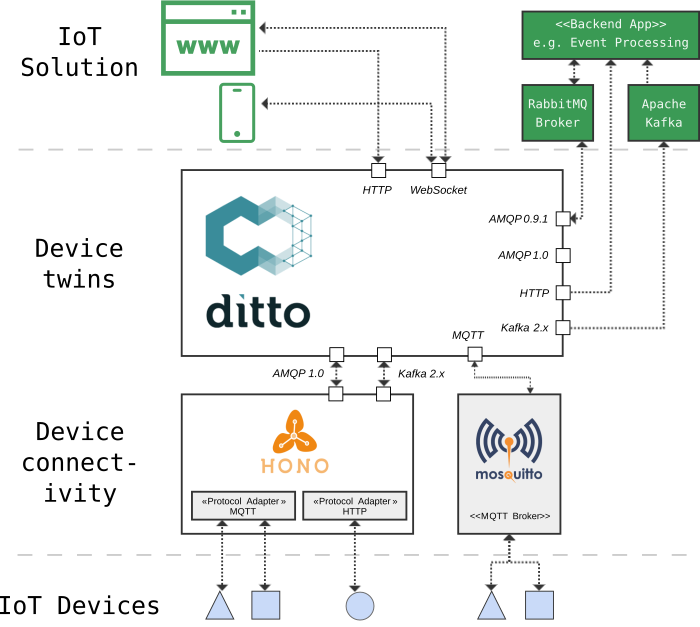
\includegraphics[width=\textwidth]{images/fp/ditto-overview-1.png}
%     \label{fig:ditto-arch}
% \end{figure}




\subsection{Implementation of ASCON and AES-GCM for device}


The implementation of both algorithms on the hardware IoT device was carried out using C and C++ programming languages within Arduino for esp-idf embedded development framework. We opted for C and C++ because those two choices are more suitable for low-level programming such as for embedded resource constraint devices. The main application for the IoT device was developed in C++, while the algorithm for ASCON and AES-GCM was implemented in C and incorporated through the use of the "extern" macro in C++ main application.


The counterpart of the algorithms in the digital twin was implemented in Java. This is because the connectivity microservice of Ditto is implemented in Java. This allowed us to extend the connectivity module using Java to incorporate an extension for encryption and decryption of the payload that comes from IoT devices.

It is worth noting that we neither altered nor introduced optimizations in the design of these algorithms. For both algorithms (ASCON\footnote{https://github.com/ascon/ascon\_collection} and AES-GCM\footnote{https://github.com/usnistgov/Lightweight-Cryptography-Benchmarking/tree/main /implementations/\_reference\_/crypto\_aead/aes-gcm/mbedtls}), we selected the optimized reference implementations tailored for the ESP32 device chip. However, to enhance the security of our implementation, we incorporated a function to generate a nonce. This aspect is crucial in addressing vulnerabilities such as replay attacks, which involve the repeated use of encrypted information.








\subsection{Ditto Java Base Payload Mapping}

In the context of Eclipse Ditto, data storage and transfer are facilitated through a format known as the Ditto protocol. This protocol utilizes a JSON structure, employing key-value pairs to represent and transmit information.

To seamlessly integrate with Ditto's capabilities, the connectivity microservice bundled with Ditto offers an extension specifically designed for intercepting incoming data. This extension allows for the mapping of data from its original form to a format that Ditto can understand and store in its underlying MongoDB database. Using the Ditto payload mapping feature, we can decrypt incoming encrypted payload messages and convert them into a format that Ditto can process and store.
 
With the payload mapping feature in Ditto's connectivity microservice, we can do the following: receive encrypted data from the IoT device, decrypt and authenticate it, and convert it into Ditto protocol messages. This helps ensure that the data sent between the IoT device and Ditto is secure and authentic.

To implement our custom mapping functionality to encrypt and decrypt, we perform the following steps:
\begin{itemize}
    \item[-] Implement and build a Java class as Jar file for the encryption and decryption functionality. This class will provide the ASCON or AES-GCM encryption and decryption operations needed for secure communication and data handling. 
    \item[-] Develop a custom message mapper class that will handle the conversion of incoming device messages to the appropriate Ditto protocol format. This class will integrate with the aforementioned encryption and decryption functionality to ensure data integrity and security during the mapping process.
    \item[-]Configure the Ditto connectivity microservice to recognize and load our custom message mapper. This configuration step ensures that incoming messages are routed to our custom mapper for processing, enabling seamless integration of our specific data transformation requirements within the Ditto framework.
\end{itemize}









\subsection{Sending Authenticated Encrypted Payload To Ditto}
\label{sec:sendingauth}

This section demonstrates the proof of concept securing the communication between the IoT device and the Digital Twin (Ditto). 

Figure \ref{fig:log-mon} depicts a snapshot captured from the serial monitor output of the board (device) utilizing PlatformIO (embedded development framework). The image showcases the device transmitting an encrypted payload to the 'ut-sensors' topic while including additional data labeled as 'tid' to uniquely identify the device. 

In Figure \ref{fig:wireshark}, a captured packet during the communication is displayed. Upon observation, it becomes evident that the topic being utilized is 'ut-sensors', and the message section of the MQTT protocol header contains the device identifier along with the encrypted payload.


\begin{figure}[H]
   
    \begin{subfigure}[c]{1\linewidth}
        \centering
        
        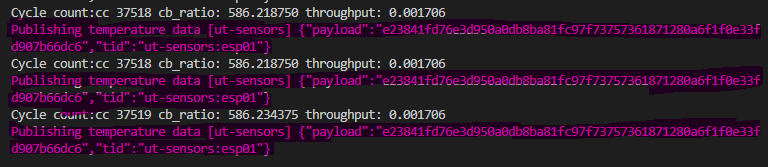
\includegraphics[width=\linewidth]{images/fp/serialport.png}
        \caption{Log Output of ESP32 Device Using Serial Monitor}
        \label{fig:log-mon}
     \end{subfigure}    

    \begin{subfigure}[c]{1\linewidth}
        \centering
        
        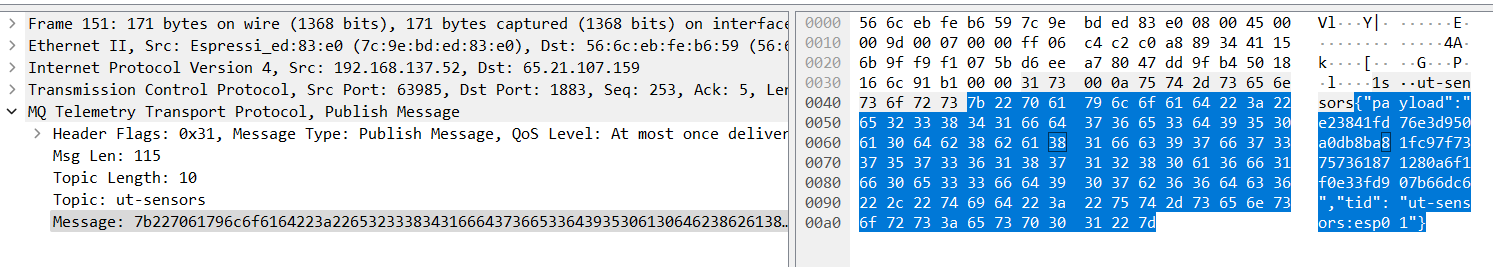
\includegraphics[width=\linewidth]{images/fp/wireshark.png}
        \caption{Wireshark Captured MQTT Communication From IoT to Ditto}
        \label{fig:wireshark}
    \end{subfigure}
     \caption{Serial Monitor of ESP32 Board and Wireshark Capturing Communication Between The Device and Ditto(DT)}
\end{figure}

The MQTT broker, hosted on the same server with Ditto, acts as a proxy, facilitating the transmission of authenticated and encrypted payloads through a publish-subscribe model. Once the MQTT broker receives a payload, it  notifies Ditto of the new message it has subscribed to. Ditto then retrieves the payload, decrypts it, and maps it into a Ditto protocol message, which is subsequently stored in a database.

To simulate the life cycle of a Digital Twin, we have developed a small web application that models the temperature and humidity features of an ESP32 sensor. The application utilizes JavaScript to retrieve these values through a stream of emissions using server-side events (SSE). Moreover, to send commands or messages to the server, we employ the HTTP POST API of Ditto. By subscribing to the command event associated with a specific topic, any device can consume the message and execute the corresponding action. This activity effectively simulates the communication between the digital twin and the actuators. Conversely, the communication from the (I)IoT device to the Digital Twin serves the purpose of collecting telemetry data from the operational environment.

\begin{figure}[H]
   
    \begin{subfigure}[c]{1\linewidth}
        
        \centering
        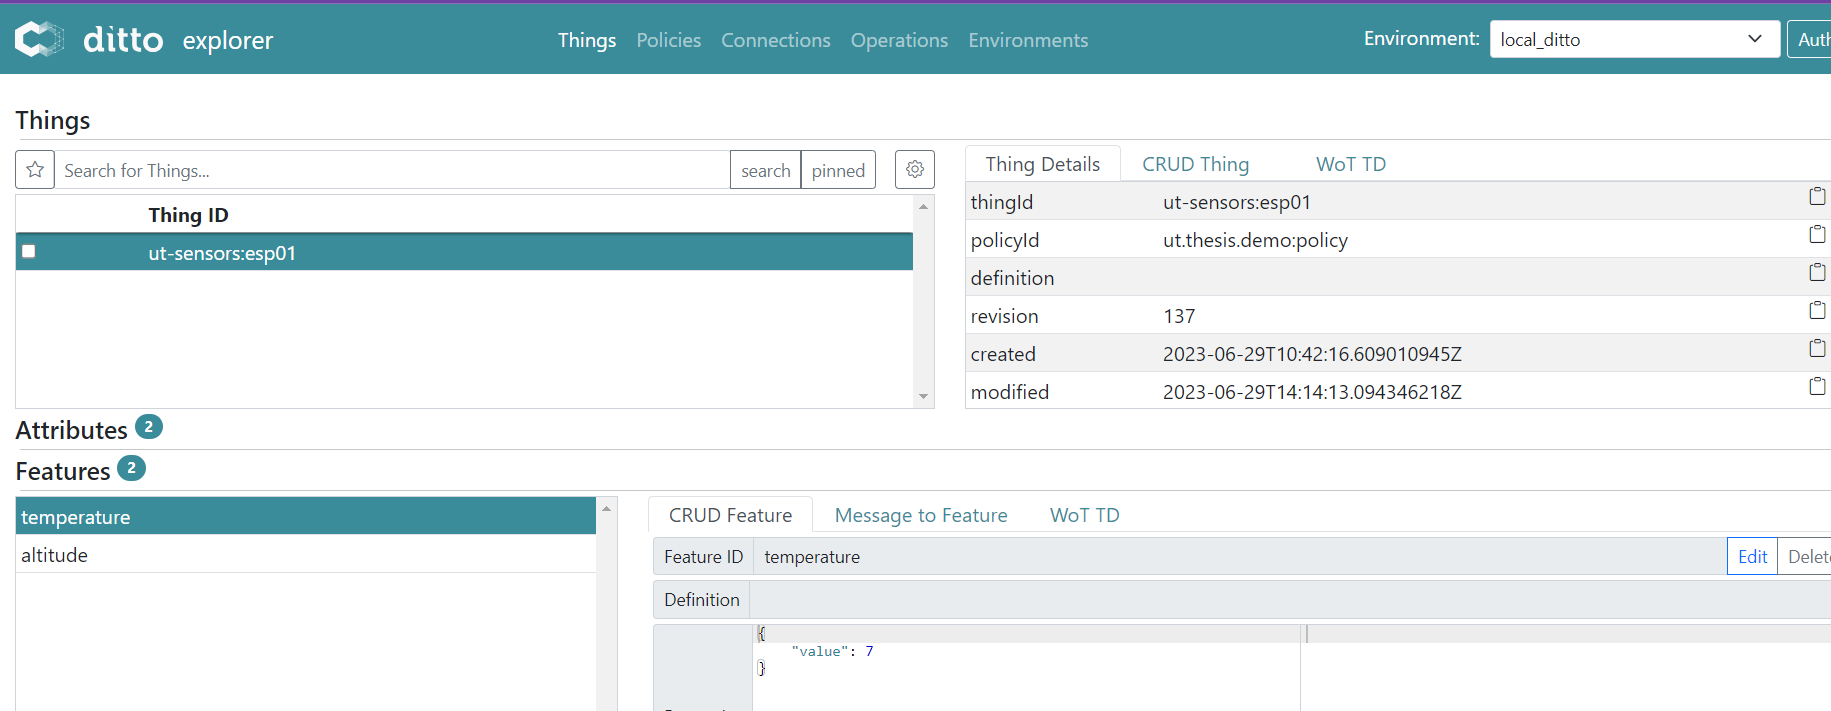
\includegraphics[width=\linewidth]{images/fp/ditto-log.png}
        \caption{A Data Log Viewed from Ditto Platform}
        \label{fig:ditto-log}
    \end{subfigure}
    
    \begin{subfigure}[c]{1\linewidth}
        \centering
        
        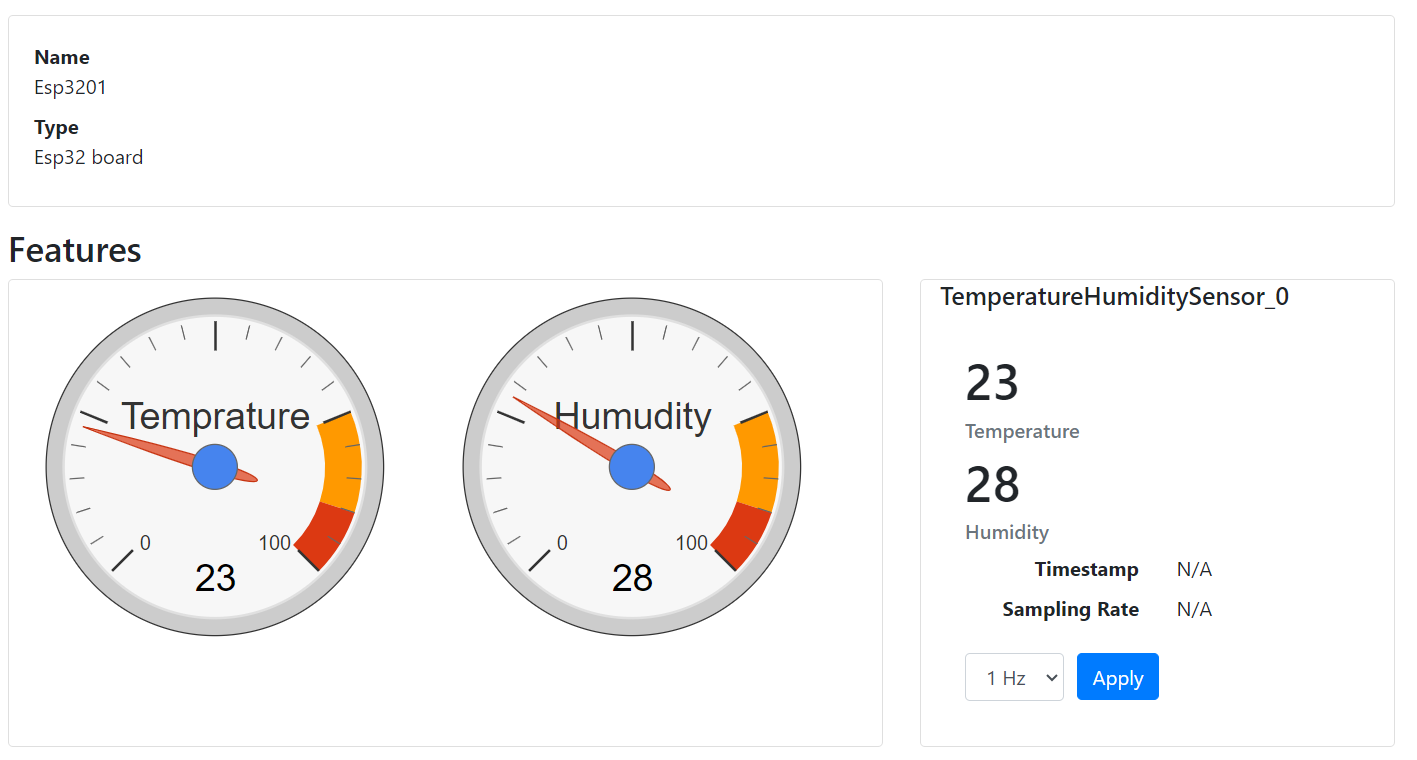
\includegraphics[width=\linewidth]{images/fp/appgauge.png}
        \caption{Web Application For Modeling Temperature and Humidity of ESP32}
        \label{fig:appdt}
     \end{subfigure} 
      \caption{Ditto and Webapp Toward Simulating Digital Twin}
    \label{fig:ditto-app}
\end{figure}

Figure \ref{fig:ditto-log} illustrates the WebUI of Ditto, which is included by default in the code base. This web portal serves as a portal offering device, policy, and connection management functionalities. Additionally, Figure \ref{fig:appdt} provides an overview of an application layer built on the Digital Twin concept. The attributes displayed on the upper part of the image represent the name and type of the simulated device. The gauges visually represent the received device features, while the bottom right section presents textual information associated with the device.

 
In this chapter, we discussed the relevant background information, the design requirement of the proposed solution and the implementation details. By implementing the proposed solution on both the Digital Twin (Ditto) and (I)IoT device (ESP32) we show how to secure the communication channel using a resource-efficient authenticated encryption algorithm. 

In the next chapter, we provided performance analysis results of our proposed solution in terms of speed, memory usage and power consumption. For the analysis, we measure the performance of three implementations which are without an encryption algorithm, with ASCON, the recent winner of NIST lightweight encryption competition, and AES-GCM, AES-based authenticated encryption with associated data algorithm. 





